\documentclass[a4, 12pt, titlepage]{scrartcl}

\usepackage[french]{babel}
% \usepackage{fontspec}
% \setmainfont{EB Garamond}[Numbers={Proportional, OldStyle},
% RawFeature={+ss06}, ItalicFeatures={Ligatures=Rare}]
\usepackage{hyperref}
\usepackage{amsmath}
\usepackage{amssymb}
\usepackage{verbatim}

\usepackage{float}

\usepackage{epigraph}

\usepackage{url}

\usepackage{graphicx}


% prettier greek letters
\renewcommand{\phi}{\varphi}
\renewcommand{\epsilon}{\varepsilon}

% sets
\newcommand{\N}[0]{\mathbb{N}}
\newcommand{\Z}[0]{\mathbb{Z}}
\newcommand{\Q}[0]{\mathbb{Q}}
\newcommand{\R}[0]{\mathbb{R}}

\newcommand{\qed}[0]{\begin{flushright} $\Box$ \end{flushright}}

\newcommand{\ie}[0]{\textit{i.e.}}

% relation symbols
\newcommand{\rel}[0]{\mathcal{R}}

% calligraphic letters
\newcommand{\Mc}[0]{\mathcal{M}}
\newcommand{\Nc}[0]{\mathcal{N}}
\newcommand{\Lc}[0]{\mathcal{L}}
\newcommand{\Uc}[0]{\mathcal{U}}
\newcommand{\Pc}[0]{\mathcal{P}}

\newcommand{\fouine}[0]{\texttt{fouine}}

\setlength{\epigraphwidth}{0.6\textwidth}

\addtokomafont{disposition}{\rmfamily}

\title{\textsc{FouineJN}, un langage Jovial et Naturel}
\subtitle{or How I learned to stop worrying and love CPS}
\author{Robin \bsc{Jourde} \& Nicolas \bsc{Nardino}}
\date{mai 2021}

\begin{document}

\maketitle

\begin{center}
  \small
  \verbatiminput{fouine-ascii.txt}
\end{center}

\newpage

\epigraph{
À l'origine fut la vitesse, la pure programmation fonctionnelle, le
<<~$\lambda x.e$~>>

Puis l'évaluation décéléra, prit consistance et forme, jusqu'aux lenteurs
habitables, jusqu'au \texttt{let}, jusqu'à vous.

Bienvenue à toi, lente fouine liée, poussif tresseur de fonctions
récursives.}{\cite{LaHorde}}




\tableofcontents

\section{Présentation}\label{sec:1}

Foino (Martes foina) aŭ estas specio de marteso kiu havas brilan
blugrizan ĝis blubrunan hararon, iom malpli delikatan ol tiu de la
arbara marteso; duobla makulo sur la gorĝo estas blanka.~\cite{wiki:001}

\fouine\ est un interpréteur de \textsc{FouineJN} (Fouine
Joviale et Naturelle~\footnote{[Citation~Needed]}), sous-ensemble du
langage de programmation national, \textsc{OCaml}.

\fouine\ est programmé principalement \textsc{OCaml} (\ref{fig:ocaml}),
et le parser associé est généré avec \textsc{Menhir} (\ref{fig:menhir}).

\begin{figure}[H]
  \centering
  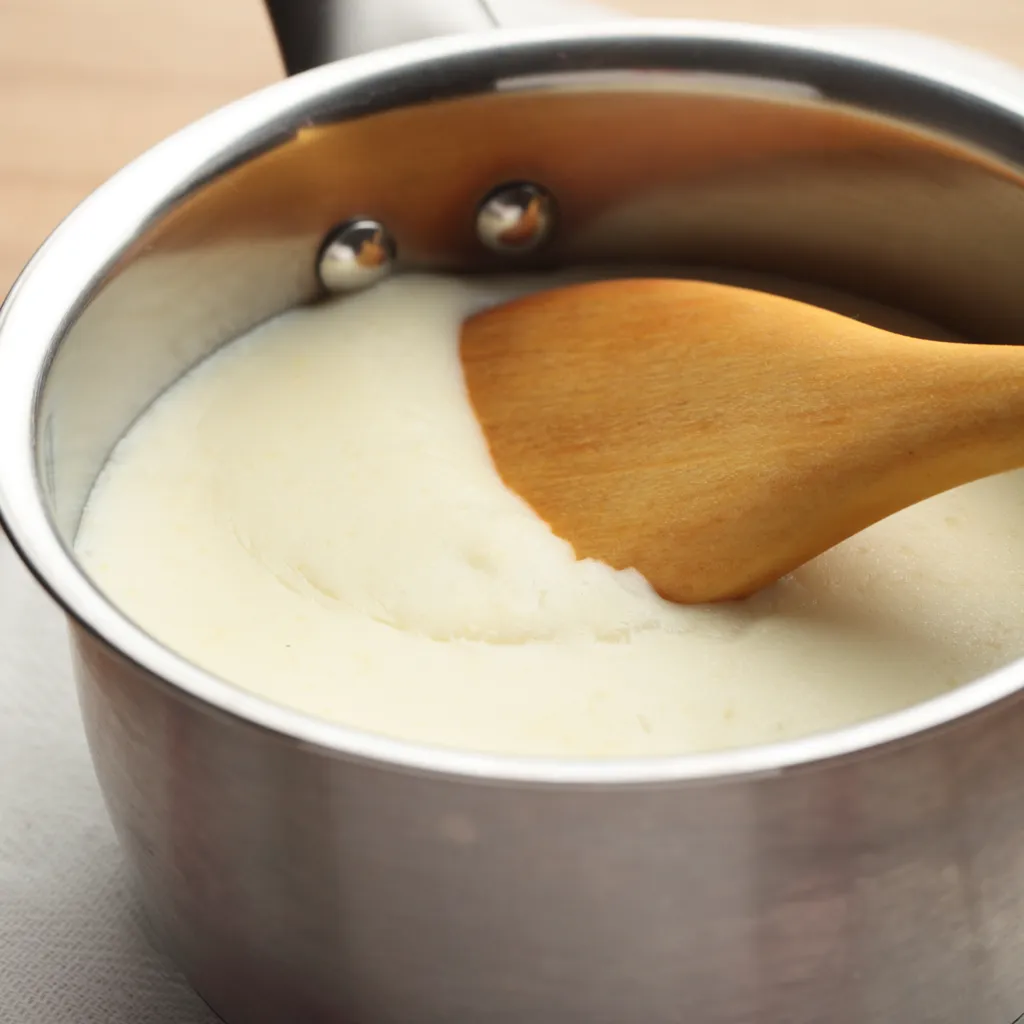
\includegraphics[width=0.33\linewidth]{figures/bechamel.png}
  \caption{\label{fig:ocaml} Exemple de béchamel, dans laquelle on
    peut trouver \texttt{caml}}
\end{figure}

\begin{figure}[H]
  \centering
  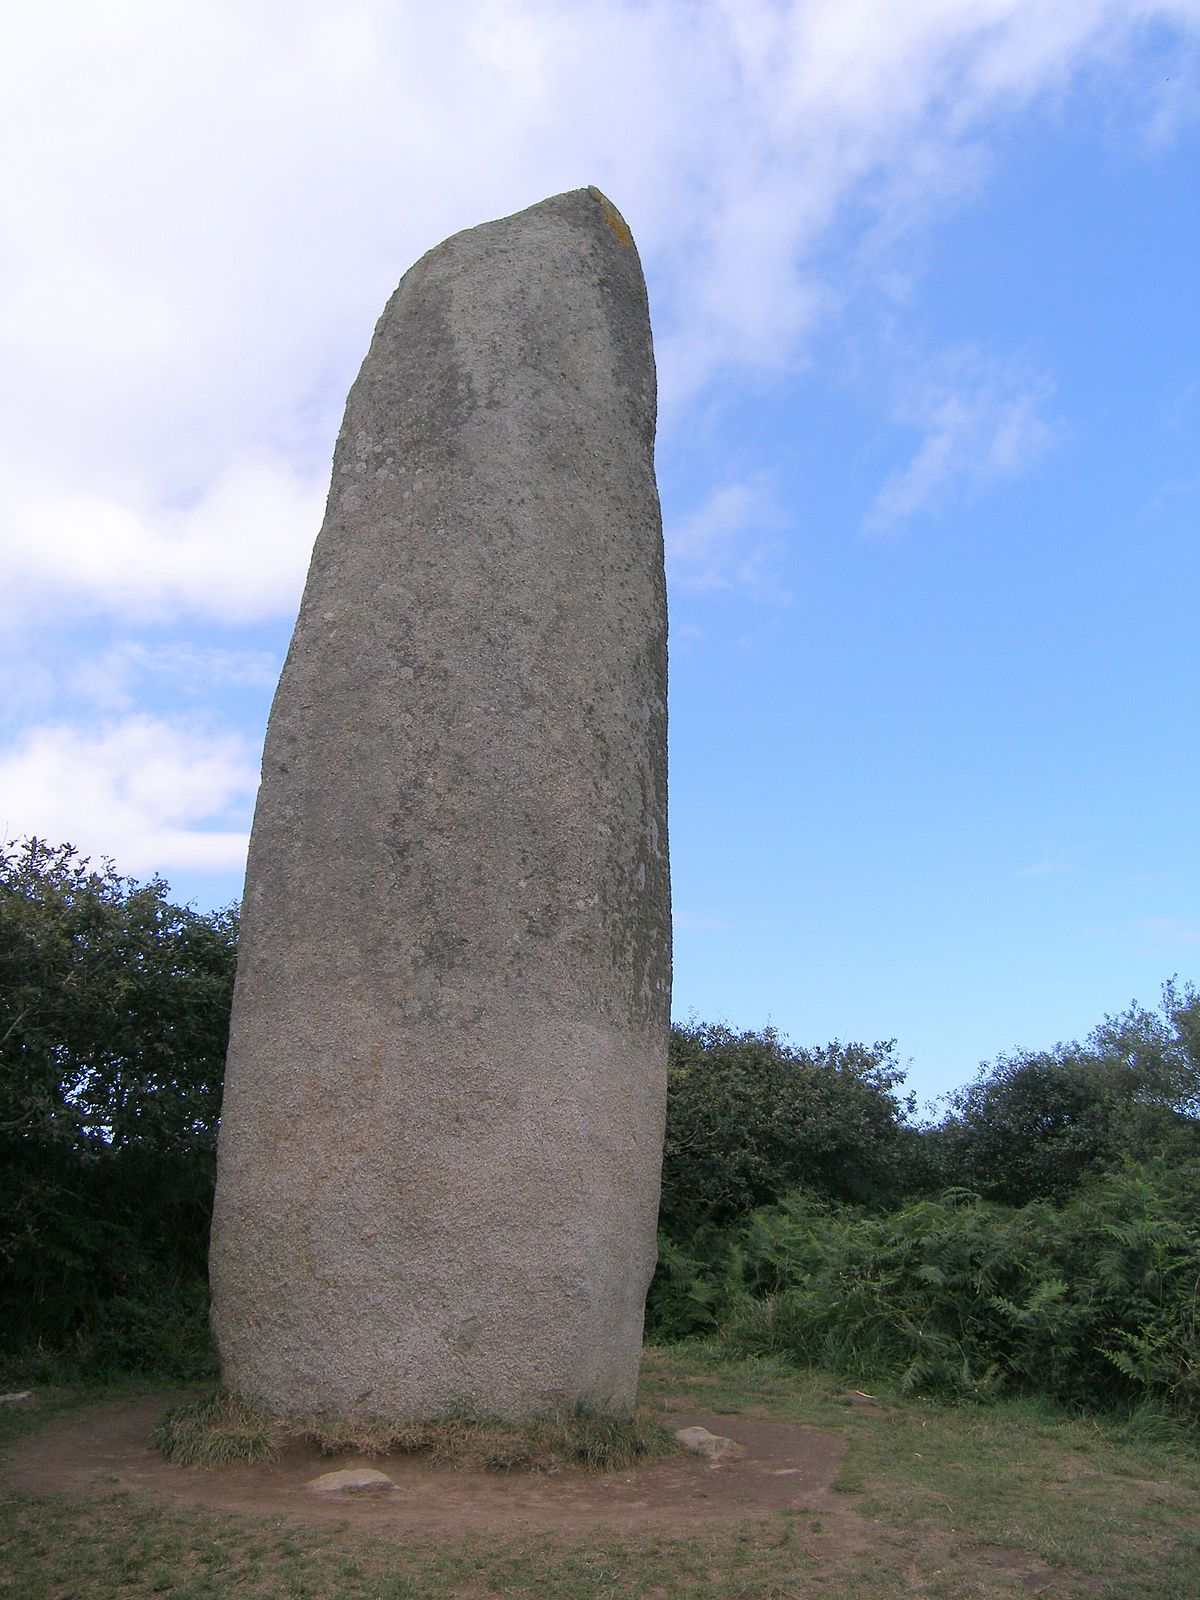
\includegraphics[width=0.33\linewidth]{figures/menhir.JPEG}
  \caption{\label{fig:menhir} Exemple de menhir}
\end{figure}

\section{Organisation et répartition du travail}\label{sec:2}

\subsection{Organisation}\label{subsec:21}


Comme dit plus haut, \fouine\ est prorammé principalement en
\textsc{OCaml}, avec pas moins de 12 fichiers
\texttt{.ml}\footnote{Source: \texttt{ls -al | grep -c "\textbackslash
    .ml\$"}}~! Nous les détaillerons plus tard. Ils sont accompagnés
d'un \texttt{lexer.mll} et \texttt{parser.mly}, qui à eux deux,
spécifient la grammaire de \textsc{FouineJN}.

Dans un ordre peu ou prou chronologique, les fichiers \texttt{.ml}
sont~:
\begin{description}
\item[expr.ml] La base de la pyramide, c'est ici qu'on définit les
  expressions.
\item[eval.ml] Le cœur du travail, c'est là que la fouine travaille
\item[main.ml] L'enrobage
\item[affichage.ml] Parce que c'est pratique d'avoir un retour sur ce
  qui se passe
\item[memory.ml] Pouvoir se souvenir de choses est un avantage
  évolutif certain, pas étonnant qu'une fouine en bénéficie
\item[stdLib.ml] Des fonctions tout plein (en particulier, nos
  opérateurs infixes)
\item[transformation.ml] Gère le transformation CPS des programmes en
  entrée
\item[reduction.ml] Aide le fichier précédent dans sa quète
\item[types.ml] On type enfin notre langage~! Analogue de
  \texttt{expr.ml}
\item[inference.ml] L'inférence de type monomorphe
\item[polymorphisme.ml] blablabla polymorphe
\item[unification.ml] Ze algorithme of unification!
\end{description}

Un, deux, trois\ldots\ Douze~! Le compte y est.

\subsection{La répartition}\label{subsec:22}

Au commencement, il n'y avait rien\ldots\ Enfin, il y avait le
mini-projet de \textsc{Proj1} de N. (noms masqués pour préserver
l'anonymité), qui a peut-être un peu aidé. Mais le vaillant R. dit~:
<<~Que les expressions soient~>> et les expressions furent. Et avec
ces dernières, l'évaluation.

Mais travailler avec des expressions brutes, ce n'est pas pratique, et
alors N. parsa. Et parsa. Et parsa. Et il vit que le parser était bien
(\emph{spoiler alert}, il n'était pas si bien que ça).

Quand vint le filtrage, un singulier shift/reduce conflict nous
embêta des semaines durant. Il s'agissait de pouvoir imbriquer deux
\texttt{match}. Jusqu'au jour de la Libération, quand le
sage D.H. nous en libéra.

Entretemps, les continuations arrivèrent, et R. entreprit de
métamorphoser ce que les vils utilisateurs envoyaient à notre
bien-aîmée \fouine\ en CPS, tandis que N. passait \texttt{eval} en
CPS, afin de pouvoir traiter les exceptions. La transformation posa
quelques problèmes à R., notamment pour les fonctions récursives, et
il dut utiliser la ruse afin de triompher (\ie\ des réductions).

Mais le triomphe fut court, et le typage pointa le bout de sa
truffe. Alors que N. inférait monomorphiquement, R. unifiait les
peuples sous sa banière, et quand ce fut fait, et que le calme
retomba, N. put enfin s'atteler aux réparations tant attendues du
parser, alors que R. s'adonna à son chef-d'œuvre, le \emph{plusieurs-formes}.

\section{Collaboration}\label{sec:3}

\subsection{git}\label{subsec:31}

Il était évident que du contrôle de version allait être nécessaire,
ainsi qu'un dépôt distant. Nous avons donc créé un dépôt sur
\texttt{github}, que l'on peut retrouver ici~:
\url{github.com/vecteurNabla/proj2}.

Grâce à notre sens de l'organisation hors du commun, notre répartition
exemplaire du travail, ainsi que qu'une bonne dose de chance sûrement,
il n'y eu que très peu de conflits à résoudre, et tous furent résolus
aisément, dans le plus grand professionnalisme, non sans l'aide de
porcelaines comme \texttt{magit}\footnote{\url{https://magit.vc/}}

\subsection{Postérité}\label{subsec:32}

Notre projet est extrêmement populaire, comme le montre le graphique
suivant~:

\begin{figure}[H]
  \centering
  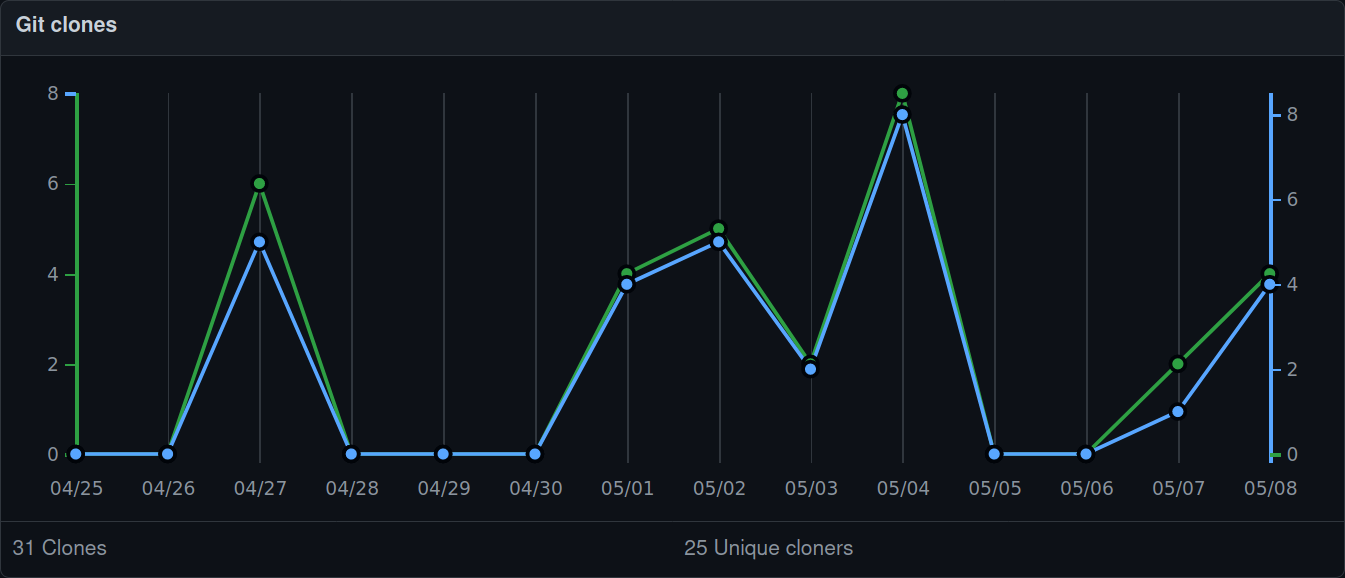
\includegraphics[width=\linewidth]{figures/clones.png}
  \caption{\label{fig:clones} Oh c'est joli c'est bleu}
\end{figure}

On peut observer pas moins de 31 clones en deux semaines~!

\cite{Landin66}.



\bsc{Tchana2025}~\cite{Tchana21}


\bibliographystyle{alpha}
\bibliography{biblio}

\end{document}
